\documentclass{exam}
\usepackage[utf8]{inputenc}
\usepackage{lmodern}
\usepackage{microtype}

% \usepackage[parfill]{parskip}
\usepackage[dvipsnames]{xcolor}
\usepackage{amsmath}
\usepackage{amsfonts}
\usepackage{amsthm}
\usepackage{siunitx}
\DeclareSIUnit\year{yr}
\DeclareSIUnit\foot{ft}
\DeclareSIUnit\litre{\liter}

\usepackage{skull}

\usepackage{pgfplots}
\usepgfplotslibrary{polar}
\pgfplotsset{compat=1.11}
\usepgfplotslibrary{statistics}
\usepackage{graphicx}
\usepackage{sidecap}
\sidecaptionvpos{figure}{c}
\usepackage{float}
\usepackage{gensymb}
\usepackage{tkz-euclide}
\usetkzobj{all}
\usepackage{commath}
\usepackage{hyperref}
\usepackage{enumitem}
\usepackage{wasysym}
\usepackage{multicol}
\usepackage{mathtools}
\usepackage{tcolorbox}
\usepackage{tabularx}
\usepackage[version=4]{mhchem}
\usepackage{changepage}
\usepackage{listings}
\lstset{basicstyle=\ttfamily\linespread{0.8}\small}

\renewcommand*{\thefootnote}{\fnsymbol{footnote}}

\newtheorem*{thm}{Theorem}
\newtheorem*{iden}{Identity}
\newtheorem*{lemma}{Lemma}
\newtheorem{obs}{Observation}
\theoremstyle{definition}
\newtheorem*{defn}{Definition}
\newtheorem*{ex}{Example}
\newtheorem{con}{Construction}
\newtheorem*{alg}{Algorithm}

\newtheoremstyle{break}
  {\topsep}{\topsep}%
  {\itshape}{}%
  {\bfseries}{}%
  {\newline}{}%
\theoremstyle{break}
\newtheorem*{bthm}{Theorem}

% russian integral
\usepackage{scalerel}
\DeclareMathOperator*{\rint}{\scalerel*{\rotatebox{17}{$\!\int\!$}}{\int}}

% \DeclareMathOperator*{\rint}{\int}

\pgfplotsset{vasymptote/.style={
    before end axis/.append code={
        \draw[densely dashed] ({rel axis cs:0,0} -| {axis cs:#1,0})
        -- ({rel axis cs:0,1} -| {axis cs:#1,0});
    }
}}

% \pointsinrightmargin
\boxedpoints
\pointname{}

\newcommand{\questioA}{\question[\texttt{\textbf{\color{Cerulean} A}}]}
\newcommand{\questioM}{\question[\texttt{\textbf{\color{PineGreen} M}}]}
\newcommand{\questioE}{\question[\texttt{\textbf{\color{WildStrawberry} E}}]}
\newcommand{\questioS}{\question[\texttt{\textbf{\color{Goldenrod} S}}]}
\newcommand{\questioO}{\question[\texttt{\textbf{\color{BurntOrange} O}}]}

\newcommand{\parA}{\part[\texttt{\textbf{\color{Cerulean} A}}]}
\newcommand{\parM}{\part[\texttt{\textbf{\color{PineGreen} M}}]}
\newcommand{\parE}{\part[\texttt{\textbf{\color{WildStrawberry} E}}]}
\newcommand{\parS}{\part[\texttt{\textbf{\color{Goldenrod} S}}]}
\newcommand{\parO}{\part[\texttt{\textbf{\color{BurntOrange} O}}]}

\newcommand{\subparA}{\subpart[\texttt{\textbf{\color{Cerulean} A}}]}
\newcommand{\subparM}{\subpart[\texttt{\textbf{\color{PineGreen} M}}]}
\newcommand{\subparE}{\subpart[\texttt{\textbf{\color{WildStrawberry} E}}]}
\newcommand{\subparS}{\subpart[\texttt{\textbf{\color{Goldenrod} S}}]}
\newcommand{\subparO}{\subpart[\texttt{\textbf{\color{BurntOrange} O}}]}

\newcommand{\mainHeader}[2]{\section*{NCEA Level 2 Mathematics\\#1. #2}}
\newcommand{\mainHeaderHw}[2]{\section*{NCEA Level 2 Mathematics (Homework)\\#1. #2}}
\newcommand{\seealso}[1]{\begin{center}\emph{See also #1.}\end{center}}
\newcommand{\drills}[1]{\begin{center}\emph{Drill problems: #1.}\end{center}}
\newcommand{\basedon}[1]{\begin{center}\emph{Notes largely based on #1.}\end{center}}

\begin{document}

\mainHeaderIntg{23}{Trigonometric Substitution}
Consider the integral
\begin{displaymath}
  \rint^1_0 x^3 \sqrt{1-x^2} \dif{x}.
\end{displaymath}
There is no obvious easy substitution to simplify this integral, and integration by parts could work but will require
a lot of work with no guranteed payoff. However, recall that $ \sqrt{1 - \sin^2 \theta} = \cos \theta $; this identity
suggests that we could perhaps substitute $ x = \sin \theta $ in order to obtain $ \dif{x} = \cos \theta \dif{\theta} $ and so
\begin{align*}
  \rint^1_0 x^3 \sqrt{1-x^2} \dif{x} &= \rint^{\frac{\pi}{2}}_0 \sin^3 \theta \cos^2 \theta \dif{\theta}\\
                                     &= \rint^{\frac{\pi}{2}}_0 \sin \theta (1-\cos^2 \theta)\cos \theta \dif{\theta}\\
                                     &= \rint^{\frac{\pi}{2}}_0 (\cos^2 \theta - \cos^4 \theta) \sin \theta \dif{\theta}
\end{align*}
Now, letting $ u = \cos \theta $ we obtain
\begin{align*}
  \rint^{\frac{\pi}{2}}_0 (\cos^2 \theta - \cos^4 \theta) \sin \theta \dif{\theta} &= -\rint^{0}_{1} u^2 - u^4 \dif{u}\\
                                                                                   &= \eval{\frac{1}{3}u^3 - \frac{1}{5}u^5}_{u = 0}^{1}\\
                                                                                   &= \frac{1}{3}-\frac{1}{5} = \frac{2}{15}.
\end{align*}

Here is a table of trig substitutions:

\begin{center}
  \def\arraystretch{1.5}
  \begin{tabular}{|c|c|c|}\hline
    \textbf{Integrand} & \textbf{Substitution} & \textbf{Identity}\\\hline
    $ \sqrt{a^2 - x^2} $ & $ x = a \sin \theta $ & $ 1 - \sin^2 \theta = \cos^2 \theta $\\\hline
    $ \sqrt{a^2 + x^2} $ & $ x = a \tan \theta $ & $ 1 + \tan^2 \theta = \sec^2 \theta $\\\hline
    $ \sqrt{x^2 - a^2} $ & $ x = a \sec \theta $ & $ \sec^2 \theta - 1 = \tan^2 \theta $\\\hline
  \end{tabular}
\end{center}


\begin{ex}
  Consider $ I = \rint \frac{\dif{x}}{\sqrt{9 + x^2}} $. Let $ x = 3\tan\theta $ so $ \dif{x} = 3\sec^2\theta \dif{\theta} $ and:
  \begin{align*}
    I &= \rint \frac{3\sec^2 \theta}{3\sqrt{1 + \tan^2 \theta}} \dif{\theta} = \rint \sec \theta \dif{\theta}\\
      &= \ln(\sec \theta + \tan \theta) + C = \ln(\sec \tan^{-1} (x/3) + x/3) + C\\
      &= \ln\left( \sqrt{\left(\frac{x}{3}\right)^2 + 1} + \frac{x}{3} \right) + C.
  \end{align*}
\end{ex}

\clearpage
\subsection*{Questions}
\begin{questions}
  \questioS Find the following integrals:
    \begin{parts}
      \part $ \rint \frac{x^2 - 9}{x^3} \dif{x} $
      \part $ \rint \frac{\dif{x}}{\sqrt{x^2 + a^2}} $
      \part $ \rint^3_0 x^2(9 - x^2) \dif{x} $
      \part $ \rint^1_0 x\sqrt{1-x^4} \dif{x} $
      \part $ \rint^2_{\sqrt{2}} \frac{\dif{x}}{t^3\sqrt{t^2 - 1}} $
      \part $ \rint \frac{\sqrt{25x^2 -4}}{x} \dif{x} $
    \end{parts}
  \questioS Use the integral $ 2\rint^{-r}_r \sqrt{r^2 - x^2} \dif{x} $ to find the area of a circle of radius $ r $.
  \questioS Scholarship 2005: Find, in terms of $ r $, the area between the ellipse $ x^2 + 16(y-r)^2 = r^2 $ and
            the circle $ x^2 + y^2 = r^2 $. You may use the substitution $ x = r \sin u $ to find the integral $ \rint \sqrt{r^2 - x^2} \dif{x} $.
  \questioS By integrating, verify that
            \begin{displaymath}
              \rint^x_0 \sqrt{a^2 - t^2} \dif{t} = \frac{1}{2} a^2 \sin^{-1} \left(\frac{x}{a}\right) + \frac{1}{2} x \sqrt{a^2 - x^2}.
            \end{displaymath}
  \questioS A charged rod of length $ L $ produces a electric field at the point $ (a,b) $ given by
            \begin{displaymath}
              E(a,b) = \rint^{L - a}_{-a} \frac{\lambda b}{4\pi \varepsilon_0 (x^2 + b^2)^{3/2}} \dif{x}.
            \end{displaymath}
            Evaluate this integral to find an explicit expression for $ E(a,b) $.
  \questioO One of these integrations should be done by partial fractions and one by trig substitution. Do them both.
            \begin{displaymath}
              \rint \frac{\dif{x}}{(4x^2 + 9)^2} \quad\quad \rint \frac{x^3}{x^2 + x - 6} \dif{x}
            \end{displaymath}
  \questioS Check this working (the substitution $ x = 3\sin\theta $ is used). Find any mistakes.
            \begin{align*}
              I &= \rint \frac{\sqrt{9 - x^2}}{x^2} \dif{x} = \rint \frac{\cos^2 \theta}{\sin^2 \theta} \dif{\theta}\\
                &= \rint \frac{1 - \sin^2 \theta}{\sin^2 \theta} \dif{\theta} = \rint \csc^2 \theta -1 \dif{\theta}\\
                &= -\cot \theta - \theta = -\cot\left(\sin^{-1} (x/3)\right) - \sin (x/3)\\
                &= \frac{\sqrt{9-x^2}}{x} - \sin(x/3).
            \end{align*}
  \clearpage
  \questioS A water storage tank has the shape of a cylinder with diameter \SI{10}{\metre}. It is mounted so that the circular cross-sections
            are vertical. If the depth of the water is \SI{7}{\metre}, what percentage of the total capacity is being used?
  \questioS When writing this worksheet I went on the internet and found this. Find the mistake(s), and do the integral.
            \begin{center}
              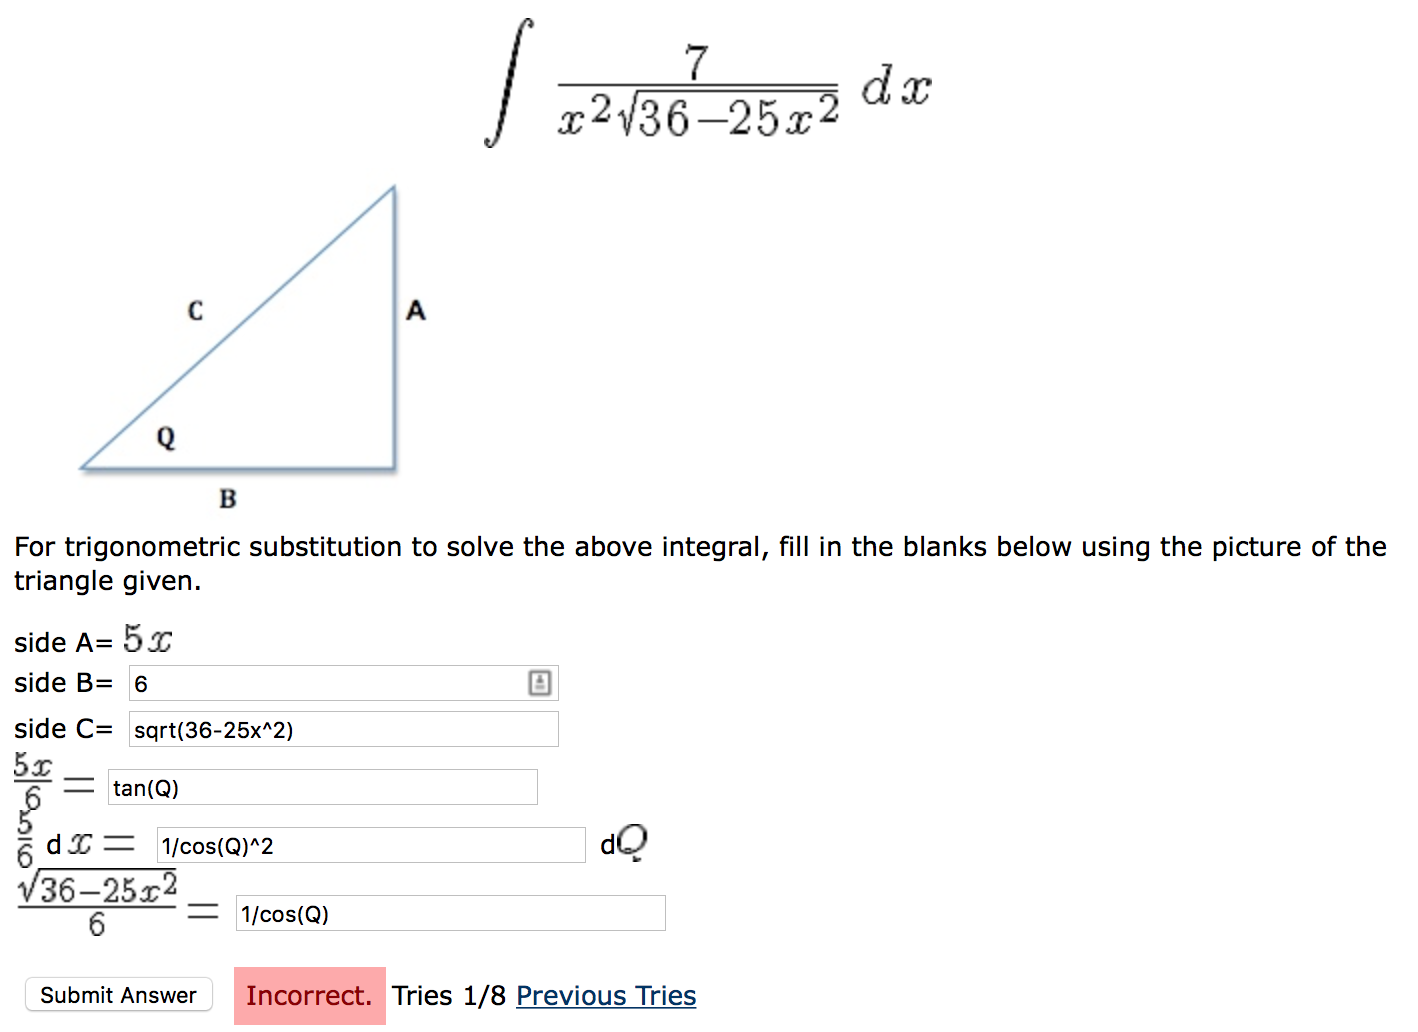
\includegraphics[width=0.7\textwidth]{misteaks1}
            \end{center}
\end{questions}
\end{document}

